\section{Longitudinal and Perpendicular Recording}
\label{sec:long-perp-record}

The magnetic grains used to store data in hard drives can be aligned such that
their easy axes (the direction in which they are most easily magnetised) point
in the direction either along (longitudinal) or perpendicular to the disk
surface. This section aims to discuss the differences between the two cases.

Most of the fundamentals of perpendicular recording were introduced in the 1970s
by Iwasaki et. al.\cite{Piramanayagam2009a} but until recently almost all hard
disk drives used longitudinal recording.  This was partly because of problems
with noise in perpendicular media which were only resolved in
2000\cite{Piramanayagam2009a} and partly because there was no need for such a
fundamental change as improvements in longitudinal recording technology allowed
for consistently increasing areal densities.

As discussed in Section~\ref{sec:hard-disk-drives}, the areal density of hard
drives is approaching a fundamental limit known as the superparamagnetic
limit. Perpendicular recording has helped to delay it in two ways. Firstly, due
to geometry it allows the same write head magnetisation to create a stronger
field in the recording medium. Secondly, it results in the bits being arranged
such that they are more likely to reinforce each others' magnetisation, giving
better stability.

The major differences between longitudinal and perpendicular recording are
illustrated in Figure~\ref{fig:Longitudinal-perpendicular}. In particular, in
perpendicular recording, the shape of the write head is changed and a soft magnetic
underlayer is added.

\begin{figure}[!ht]
  \center
  \includegraphics[width=1\textwidth]{./perp_rec/perphead}
  \caption{The write head set up for longitudinal and perpendicular recording.
    Image modified from
    \cite{LongitudinalPerpDiagram}.}
  \label{fig:Longitudinal-perpendicular}
\end{figure}

\subsection{Write Heads}

\subsubsection{Write Head Arrangements}

As shown in Figure~\ref{fig:Longitudinal-perpendicular} the write head is
arranged differently in longitudinal and perpendicular recording.

Longitudinal recording requires a \emph{ring head}. At a basic level it consists
of a ring of soft magnetic material with a coil of wire around it and a small
gap in the ring near surface of the disk. When current flows through the wire it
magnetises the ring. This magnetisation can be thought of as magnetic flux
flowing around the ring, at the gap the flux spreads out causing a ``fringing
field'' in the surrounding area. This is the field that is used to write to the
recording media.\cite{Khizroev2004a}

A similar head can be used for perpendicular recording, but because of the
orientation of the magnetisation a better option is available: a \emph{single
  pole head }(SPH). A single pole head consists of a roughly semicircular piece
of soft magnetic material with a coil around it above the disk and a \emph{soft
  magnetic underlayer} (SUL) below the recording layer.  Magnetic flux flows
around the semicircular head and directly through the recording layer before
being redirected back to the other end of the head by the soft underlayer. If
one of the poles of the head is made much narrower than the other then flux is
concentrated below the narrow pole but spread out below the other pole. This
means that only the narrow pole has a strong enough field to write to the disk
-- hence the name.\cite{Khizroev2004a}

A good way to think about the soft underlayer is to use the method of images,
similar to that used for conductors in electrostatics. \cite{Hoinville2002}
According to this method the effect of an ideal (infinitely thick with infinite
permeability) soft underlayer is the same as that of a mirror image of the real
write head (with the line of symmetry at the surface of the soft underlayer)
with ``magnetic charges'' of the opposite sign, as shown in
Figure~\ref{fig:imaginary_head}. In this approximation a single pole head with a
soft magnetic underlayer is similar to a ring head except that the writing takes
place directly within the gap rather than outside it.\cite{Richter2007a}

\begin{figure}[!ht]
  \center
  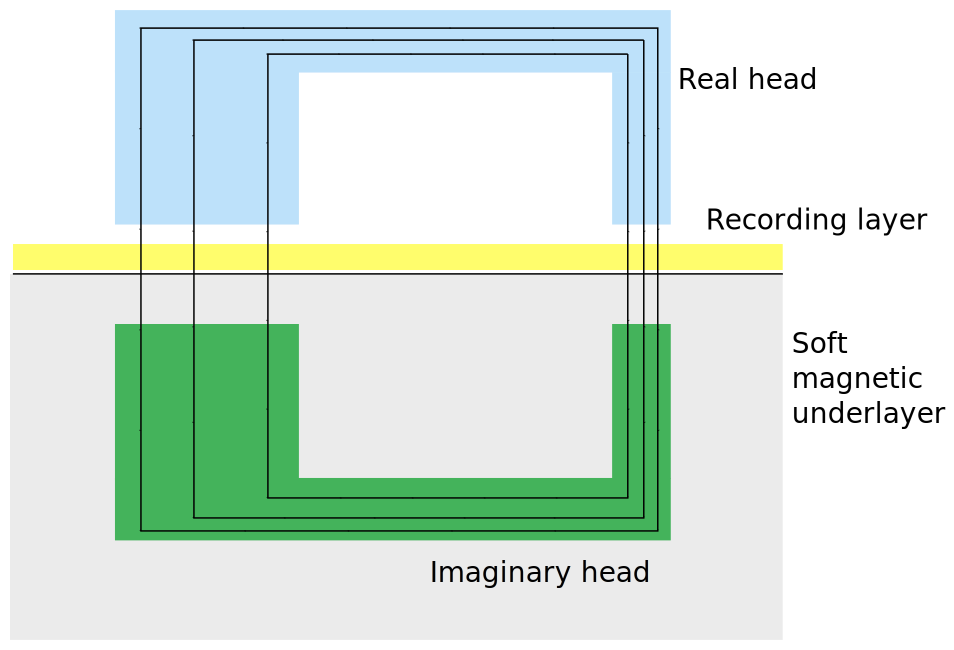
\includegraphics[width=0.75\textwidth]{./perp_rec/SPH_images}
  \caption{A single pole head along with its image in a soft magnetic underlayer
    with magnetic flux line shown.\label{fig:imaginary_head}}
\end{figure}


\subsubsection{Effects on the applied write field}

The write field (in the recording direction) at a point on the recording medium
is related to the solid angle filled by the write head (in steradians),
$\omega$, and the magnetisation of the write head in the recording direction,
$M_{z}$ by\cite{Richter2007a}
\[ H_{z}=\dfrac{M_{z} \omega}{4\pi}.\]

As a simple model we assume that the write head extends infinitely both along
and across the track (i.e. in the $x$ and $y$ directions). Then for a ring head
the solid angle is $\omega=2\pi$ sr, corresponding to the entire top hemisphere
being filled. By comparison for a single pole the solid angle is $\omega=4\pi$
sr because the top hemisphere is filled by the real head and the bottom
hemisphere is filled by the imaginary head created by the soft underlayer. Hence
in this approximation the applied field for a single pole head is double the
applied field for a ring head. Obviously real write heads are finite but single
pole heads still produce approximately double the applied field for the same
head magnetisation.\cite{Khizroev2004a} As mentioned previously in
Section~\ref{sec:trilemma} an increase in the write field allows the use of
higher anisotropy materials in the recording layer which increases the thermal
stability of bits allowing an increase in areal density.


\subsection{Magnetostatic Fields}

The magnetostatic field of a magnetised body is the field created by the body
itself. This field affects the magnetisation of the body leading to complex
interactions. The magnetostatic field is also known as the demagnetising field
(because it tends to oppose the magnetisation of the body creating it) or the
stray field. It is the cause of shape anisotropy -- the shape of a magnetic body
affects the magnetostatic field and hence can sometimes give a preferred
magnetisation direction.

A simple way to think about the magnetostatic field is to use poles. When a
piece of ferromagnetic material is magnetised poles are created at the ends
causing a magnetostatic field ($\Hms$) opposing the magnetisation within the
material. As a simple rule of thumb the strength of $\Hms$ is inversely
proportional to the separation of the magnetic poles. \cite{Piramanayagam2007a}

\begin{figure}[!ht]
  \center
  \includegraphics[width=0.8\textwidth]{./perp_rec/demagsimple}
  \caption{
    A simple picture of magnetic charges in longitudinal and perpendicular
    recording media. The thickness of the arrows show the strength of the
    internal magnetostatic field.  Modified from Piramanayagam
    2007. \cite{Piramanayagam2007a}}
  \label{fig:simple-picture-demag}
\end{figure}


\subsubsection{Differences in Internal Magnetostatic Field Between Perpendicular and Longitudinal Recording}
\label{sec:diff-intern-magn}
We first focus on the internal magnetostatic field -- the effect of the magnetisation of a body (or a bit in magnetic data storage) on itself.

Strong internal magnetostatic fields can cause problems in magnetic data storage
because they work against the anisotropy of the ferromagnetic grains, reducing
the thermal stability of the grains. This effect cannot be counteracted simply
by increasing the anisotropy because the magnetostatic field is
non-constant. Hence it is preferable to keep the internal magnetostatic fields
as small as possible.

A simple idea of the differences in internal magnetostatic field strength between
longitudinal and perpendicular recording can be seen by examining the
distribution of magnetic poles. A comparison of the two is shown in Figure
\ref{fig:simple-picture-demag}. For low linear data densities (i.e. large bit areas)
and thin films longitudinal recording has a larger separation of the magnetic
poles that cause the internal magnetostatic field, hence longitudinal recording has a
lower internal magnetostatic field. At high linear data densities and/or thicker films
perpendicular recording gives a lower internal magnetostatic field for the same
reason.\cite{Piramanayagam2007a}

\begin{figure}[!ht]
  \center
  \includegraphics[width=1\textwidth]{./perp_rec/perpvslongdemags}
  \caption{Calculated magnetostatic fields near a single ideal transition for
    longitudinal (left) and perpendicular (right) recording. The perpendicular
    recording calculation assumes an ideal soft underlayer. The grey line on each
    graph corresponds to a thicker magnetic recording layer. Modified from Litvinov
    2002\cite{Litvinov2002}.}
  \label{fig:Calculated-demagnetising-fields}
\end{figure}

The magnetostatic fields can be more precisely calculated from the magnetic
charge distributions. Plots of these calculations of the magnetostatic fields at
the centre of the recording layer near an ideal transition (a change in the
magnetisation direction) are shown in Figure
\ref{fig:Calculated-demagnetising-fields}. It can be seen that the field
decreases near the point of the transition for the perpendicular case whereas
for the longitudinal case it reaches a maximum. This implies a lower
magnetostatic field for perpendicular recording at short bit lengths (i.e. high
areal density). Also the magnetostatic field decreases for thicker recording
layers in perpendicular recording while the opposite happens in the longitudinal
case. Hence this more advanced description agrees with the simple explanation
given above.\cite{Litvinov2002}

In the case that neighbouring tracks have opposite magnetisation the
magnetostatic field also decreases with track density. However encoding data to
arrange this scenario causes too large a decrease in storage capacity to be
useful. \cite{Litvinov2002}

\begin{figure}
  \begin{center}
    \hspace{-5em} % Manual centering...
    % GNUPLOT: LaTeX picture with Postscript
\begingroup
  \makeatletter
  \providecommand\color[2][]{%
    \GenericError{(gnuplot) \space\space\space\@spaces}{%
      Package color not loaded in conjunction with
      terminal option `colourtext'%
    }{See the gnuplot documentation for explanation.%
    }{Either use 'blacktext' in gnuplot or load the package
      color.sty in LaTeX.}%
    \renewcommand\color[2][]{}%
  }%
  \providecommand\includegraphics[2][]{%
    \GenericError{(gnuplot) \space\space\space\@spaces}{%
      Package graphicx or graphics not loaded%
    }{See the gnuplot documentation for explanation.%
    }{The gnuplot epslatex terminal needs graphicx.sty or graphics.sty.}%
    \renewcommand\includegraphics[2][]{}%
  }%
  \providecommand\rotatebox[2]{#2}%
  \@ifundefined{ifGPcolor}{%
    \newif\ifGPcolor
    \GPcolorfalse
  }{}%
  \@ifundefined{ifGPblacktext}{%
    \newif\ifGPblacktext
    \GPblacktexttrue
  }{}%
  % define a \g@addto@macro without @ in the name:
  \let\gplgaddtomacro\g@addto@macro
  % define empty templates for all commands taking text:
  \gdef\gplbacktext{}%
  \gdef\gplfronttext{}%
  \makeatother
  \ifGPblacktext
    % no textcolor at all
    \def\colorrgb#1{}%
    \def\colorgray#1{}%
  \else
    % gray or color?
    \ifGPcolor
      \def\colorrgb#1{\color[rgb]{#1}}%
      \def\colorgray#1{\color[gray]{#1}}%
      \expandafter\def\csname LTw\endcsname{\color{white}}%
      \expandafter\def\csname LTb\endcsname{\color{black}}%
      \expandafter\def\csname LTa\endcsname{\color{black}}%
      \expandafter\def\csname LT0\endcsname{\color[rgb]{1,0,0}}%
      \expandafter\def\csname LT1\endcsname{\color[rgb]{0,1,0}}%
      \expandafter\def\csname LT2\endcsname{\color[rgb]{0,0,1}}%
      \expandafter\def\csname LT3\endcsname{\color[rgb]{1,0,1}}%
      \expandafter\def\csname LT4\endcsname{\color[rgb]{0,1,1}}%
      \expandafter\def\csname LT5\endcsname{\color[rgb]{1,1,0}}%
      \expandafter\def\csname LT6\endcsname{\color[rgb]{0,0,0}}%
      \expandafter\def\csname LT7\endcsname{\color[rgb]{1,0.3,0}}%
      \expandafter\def\csname LT8\endcsname{\color[rgb]{0.5,0.5,0.5}}%
    \else
      % gray
      \def\colorrgb#1{\color{black}}%
      \def\colorgray#1{\color[gray]{#1}}%
      \expandafter\def\csname LTw\endcsname{\color{white}}%
      \expandafter\def\csname LTb\endcsname{\color{black}}%
      \expandafter\def\csname LTa\endcsname{\color{black}}%
      \expandafter\def\csname LT0\endcsname{\color{black}}%
      \expandafter\def\csname LT1\endcsname{\color{black}}%
      \expandafter\def\csname LT2\endcsname{\color{black}}%
      \expandafter\def\csname LT3\endcsname{\color{black}}%
      \expandafter\def\csname LT4\endcsname{\color{black}}%
      \expandafter\def\csname LT5\endcsname{\color{black}}%
      \expandafter\def\csname LT6\endcsname{\color{black}}%
      \expandafter\def\csname LT7\endcsname{\color{black}}%
      \expandafter\def\csname LT8\endcsname{\color{black}}%
    \fi
  \fi
  \setlength{\unitlength}{0.0500bp}%
  \begin{picture}(9070.00,4534.00)%
    \gplgaddtomacro\gplbacktext{%
      \csname LTb\endcsname%
      \put(946,704){\makebox(0,0)[r]{\strut{} 0}}%
      \put(946,1417){\makebox(0,0)[r]{\strut{} 0.2}}%
      \put(946,2130){\makebox(0,0)[r]{\strut{} 0.4}}%
      \put(946,2843){\makebox(0,0)[r]{\strut{} 0.6}}%
      \put(946,3556){\makebox(0,0)[r]{\strut{} 0.8}}%
      \put(946,4269){\makebox(0,0)[r]{\strut{} 1}}%
      \put(1078,484){\makebox(0,0){\strut{} 0}}%
      \put(1690,484){\makebox(0,0){\strut{} 0.2}}%
      \put(2302,484){\makebox(0,0){\strut{} 0.4}}%
      \put(2914,484){\makebox(0,0){\strut{} 0.6}}%
      \put(3526,484){\makebox(0,0){\strut{} 0.8}}%
      \put(4138,484){\makebox(0,0){\strut{} 1}}%
      \put(176,2486){\rotatebox{-270}{\makebox(0,0){\strut{}$\dfrac{-H_{m,x}}{M_s}$}}}%
      \put(2608,154){\makebox(0,0){\strut{}$\rho$}}%
    }%
    \gplgaddtomacro\gplfronttext{%
    }%
    \gplgaddtomacro\gplbacktext{%
      \csname LTb\endcsname%
      \put(5481,704){\makebox(0,0)[r]{\strut{} 0}}%
      \put(5481,1417){\makebox(0,0)[r]{\strut{} 0.2}}%
      \put(5481,2130){\makebox(0,0)[r]{\strut{} 0.4}}%
      \put(5481,2843){\makebox(0,0)[r]{\strut{} 0.6}}%
      \put(5481,3556){\makebox(0,0)[r]{\strut{} 0.8}}%
      \put(5481,4269){\makebox(0,0)[r]{\strut{} 1}}%
      \put(5613,484){\makebox(0,0){\strut{} 0}}%
      \put(6225,484){\makebox(0,0){\strut{} 0.2}}%
      \put(6837,484){\makebox(0,0){\strut{} 0.4}}%
      \put(7449,484){\makebox(0,0){\strut{} 0.6}}%
      \put(8061,484){\makebox(0,0){\strut{} 0.8}}%
      \put(8673,484){\makebox(0,0){\strut{} 1}}%
      \put(4711,2486){\rotatebox{-270}{\makebox(0,0){\strut{}$\dfrac{-H_{m,z}}{M_s}$}}}%
      \put(7143,154){\makebox(0,0){\strut{}$\rho$}}%
    }%
    \gplgaddtomacro\gplfronttext{%
    }%
    \gplbacktext
    \put(0,0){\includegraphics{external_field_at_surface}}%
    \gplfronttext
  \end{picture}%
\endgroup

    \caption{Normalised magnetostatic fields for longitudinal (left) and perpendicular (right) recording at the surface of the recording layer as a function of $\rho$ (the ratio of bit thickness to bit length).}
    \label{fig:surface-demag}
  \end{center}
\end{figure}

\subsubsection{External Magnetostatic Fields}
\label{sec:Stray-fields}

The external magnetostatic field is important in magnetic data storage because
it is the field detected by the read head when data is being read from the
disc. \cite{Richter1999}

A good measure of the strength of the field at the read head is the strength of
the internal magnetostatic field at the surface of the disk. For the case of a
sinusoidally varying magnetisation (i.e. the binary pattern 01010101) the bit
density can be written as $\rho=\dfrac{\delta}{\lambda}$ where $\lambda$ is the
wavelength of the sinusoidal variation and $\delta$ is the thickness of the recording
layer. The magnetostatic field at the surface of the disk is then
\[ H_{m,x}=-\frac{M_s}{2}(1-e^{-2\pi\rho}),\]
in the $x$ direction for the longitudinal case and
\[ H_{m,z}=-\frac{M_s}{2}(1+e^{-2\pi\rho}),\]
in the $z$ direction for the perpendicular case. \cite{Richter1999}


Figure~\ref{fig:surface-demag} shows plots of $H_{m,x}$ and $H_{m,z}$ against
$\rho$. Note that for reasonably large $\rho$ (i.e. for bits that are shorter in
length than the thickness of the recording layer) both fields approach
$H_{m}=-\dfrac{M}{2}$. For almost any realistic case the strength of the
magnetostatic field near the read head is no different between the two recording
orientations. Hence in this approximation there is no difference in signal
strength between the two types of recording media. A more detailed comparison by
Litvinov \cite{Litvinov2005a} showed that using perpendicular recording actually
gives a higher signal strength, mostly due to the soft underlayer.

\begin{figure}
  \center
  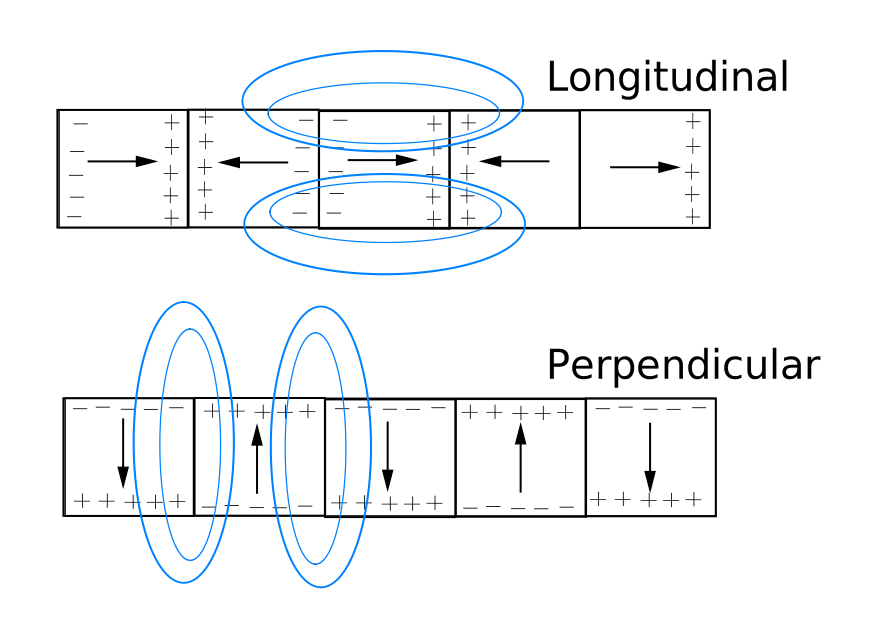
\includegraphics[width=0.8\textwidth]{./perp_rec/strayfielddiffs}
  \caption{Stray field directions in longitudinal and perpendicular
    recording.}
  \label{fig:Stray-field-directions}
\end{figure}

% you should add a citation for  "However by encoding the data we can obtain a recording that largely consists of alternating bits without too much loss of areal density, and this encoding is regularly used for other reasons'' if still in the thesis
The external magnetostatic field effects on neighbouring bits in longitudinal
and perpendicular recording are shown in Figure
\ref{fig:Stray-field-directions}. From this we can see that as long as
transitions are fairly common the magnetostatic field from nearby bits actually
reinforce each other in the perpendicular media case. Conversely, for the same
pattern, the fields created by bits in longitudinal media act against the
magnetisation of neighbouring bits. Naively this would appear to be of no use
since real data do not always form an alternating pattern. However data is
typically encoded such that it largely consists of alternating bits for other
reasons. Hence the magnetostatic fields in perpendicular recording actually
increase thermal stability of neighbouring bits but decrease stability in
longitudinal recording.


%%% Local Variables:
%%% mode: latex
%%% TeX-master: "main"
%%% End:
